\subsection*{Open Redirect -- Unvalidated Redirect Parameter (OR)}

\begin{table}[H]
\centering
\begin{tabular}{|l|p{10cm}|}
\hline
\textbf{Finding ID} & OR \\
\hline
\textbf{Severity} & Medium \\
\hline
\textbf{CVSS 3.1 Score} & 4.3 (Medium) \\
\hline
\textbf{CVSS Vector} & \texttt{AV:N/AC:L/PR:N/UI:R/S:U/C:N/I:L/A:N} \\
\hline
\textbf{Status} & Confirmed \\
\hline
\textbf{OWASP Category} & A01:2021 -- Broken Access Control \\
\hline
\textbf{CWE} & CWE-601 -- URL Redirection to Untrusted Site (Open Redirect) \\
\hline
\textbf{Affected Endpoint} & \texttt{GET /redirect} \\
\hline
\textbf{Affected Parameter} & \texttt{to} \\
\hline
\end{tabular}
\caption{Open Redirect finding details}
\end{table}

\subsubsection*{Description}

The application provides a redirect feature at \texttt{/redirect},
which takes a destination website through the \texttt{to} parameter
and automatically sends the user's browser there.

The application attempts to allow redirects only to trusted
destinations, but the validation check is not strict enough.
Instead of properly verifying the actual destination, it checks
whether a trusted domain string appears somewhere in the URL.

This allows the validation check to be bypassed by placing an
attacker-controlled destination first, followed by a trusted domain
string elsewhere in the same URL.

\subsubsection*{Methodology}

The vulnerability was first identified during the OWASP ZAP
automated scan. Manual testing was then performed to verify whether
the redirect validation could be bypassed.

A trusted redirect destination was tested first, followed by an
untrusted destination. Finally, a crafted URL containing an
attacker-controlled domain and a trusted domain string was tested.

The browser was successfully redirected to the attacker-controlled
domain, confirming the vulnerability.

\subsubsection*{Steps to Reproduce}

\begin{enumerate}

    \item Confirm that a known trusted destination redirects
    correctly:

    \begin{lstlisting}
http://127.0.0.1:3000/redirect?to=https://github.com/juice-shop/juice-shop
    \end{lstlisting}

    \item Attempt an untrusted destination directly and observe that
    it is blocked with a \texttt{406 Unrecognized target URL} error:

    \begin{lstlisting}
http://127.0.0.1:3000/redirect?to=https://www.google.com
    \end{lstlisting}

    \item Bypass the validation check by placing an
    attacker-controlled domain first, followed by a trusted domain
    string elsewhere in the URL:

    \begin{lstlisting}
http://127.0.0.1:3000/redirect?to=https://evil.com/?https://github.com/juice-shop/juice-shop
    \end{lstlisting}

    \item Observe that the browser is redirected to
    \texttt{evil.com} instead of being blocked. This confirms that
    the redirect validation can be bypassed.

\end{enumerate}

\subsubsection*{Evidence}

The following evidence demonstrates both automated detection and
manual confirmation of the vulnerability.

\begin{figure}[H]
    \centering
    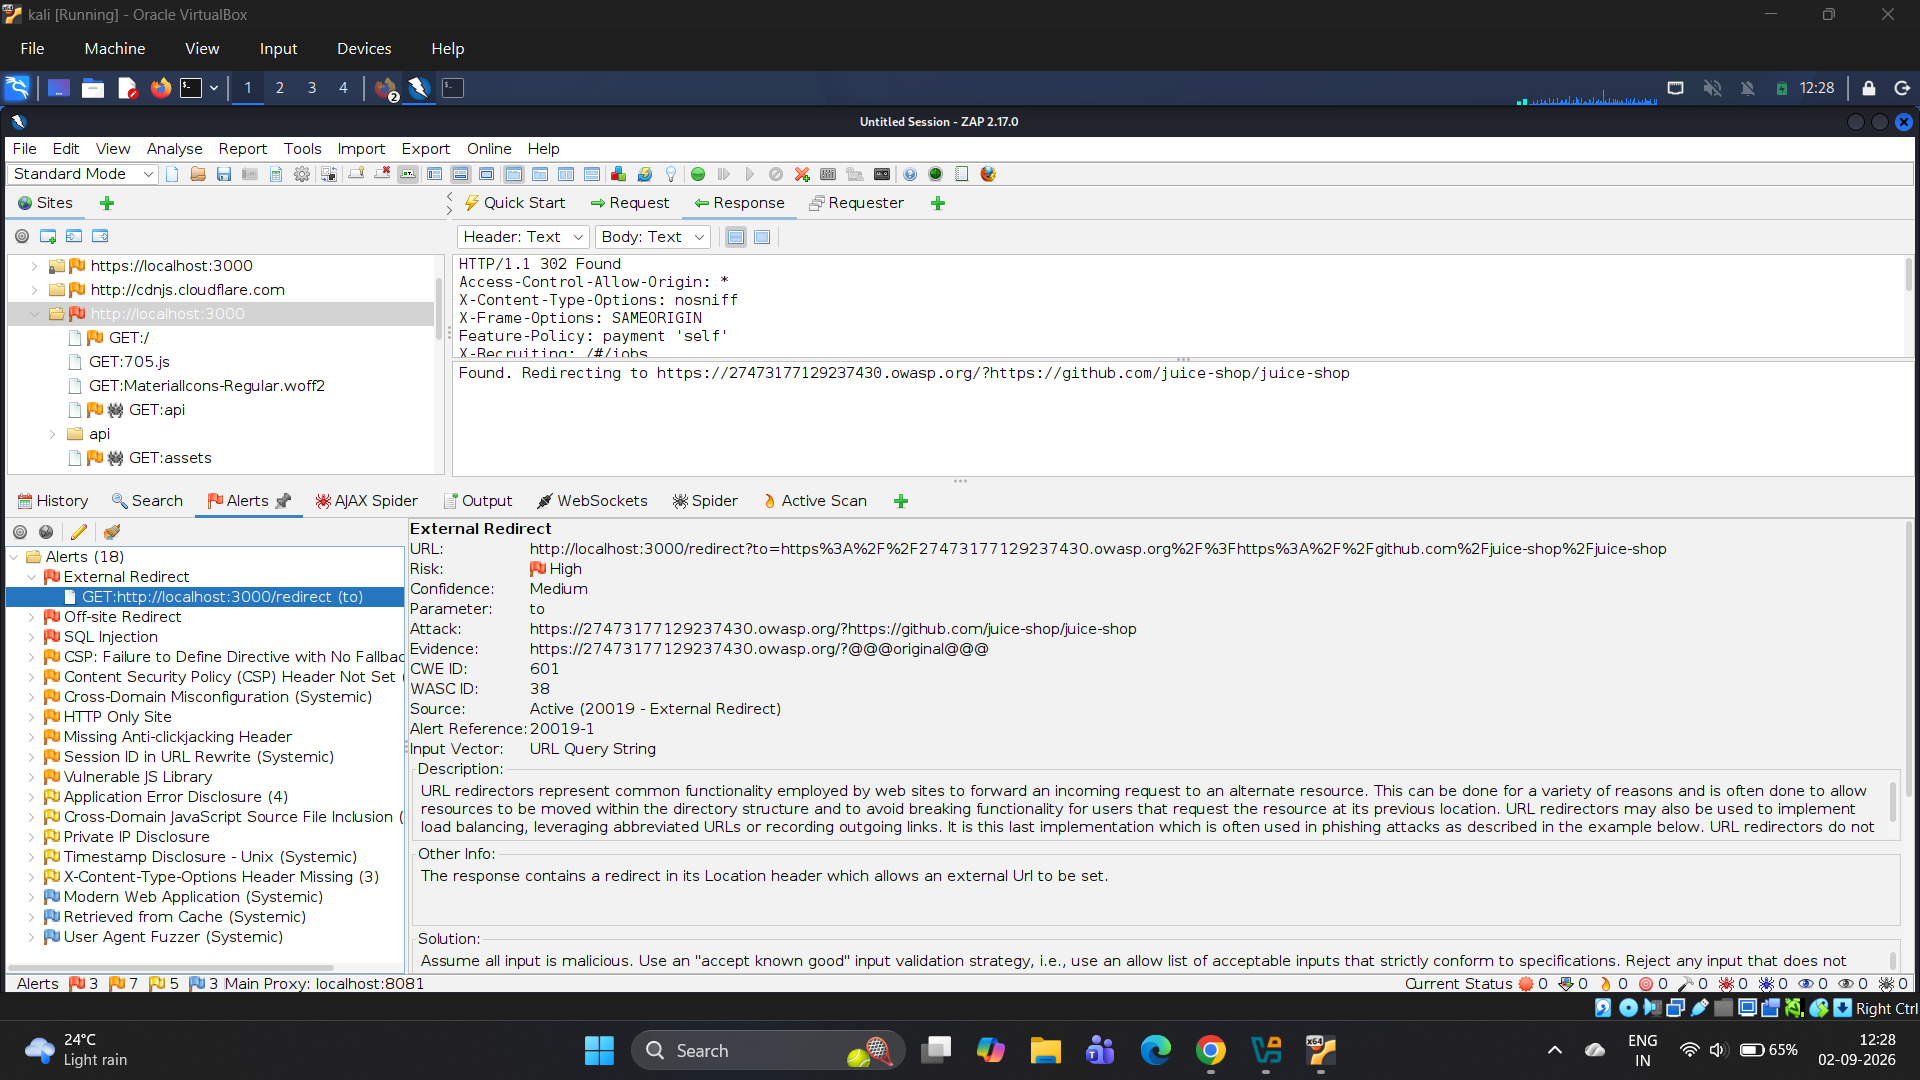
\includegraphics[width=0.8\textwidth]
    {evidence/phase3/zap/openredirect-01-zap-alert-detection.png}
    \caption{OWASP ZAP alert flagging the redirect parameter as vulnerable}
    \label{fig:openredirect-zap}
\end{figure}

\begin{figure}[H]
    \centering
    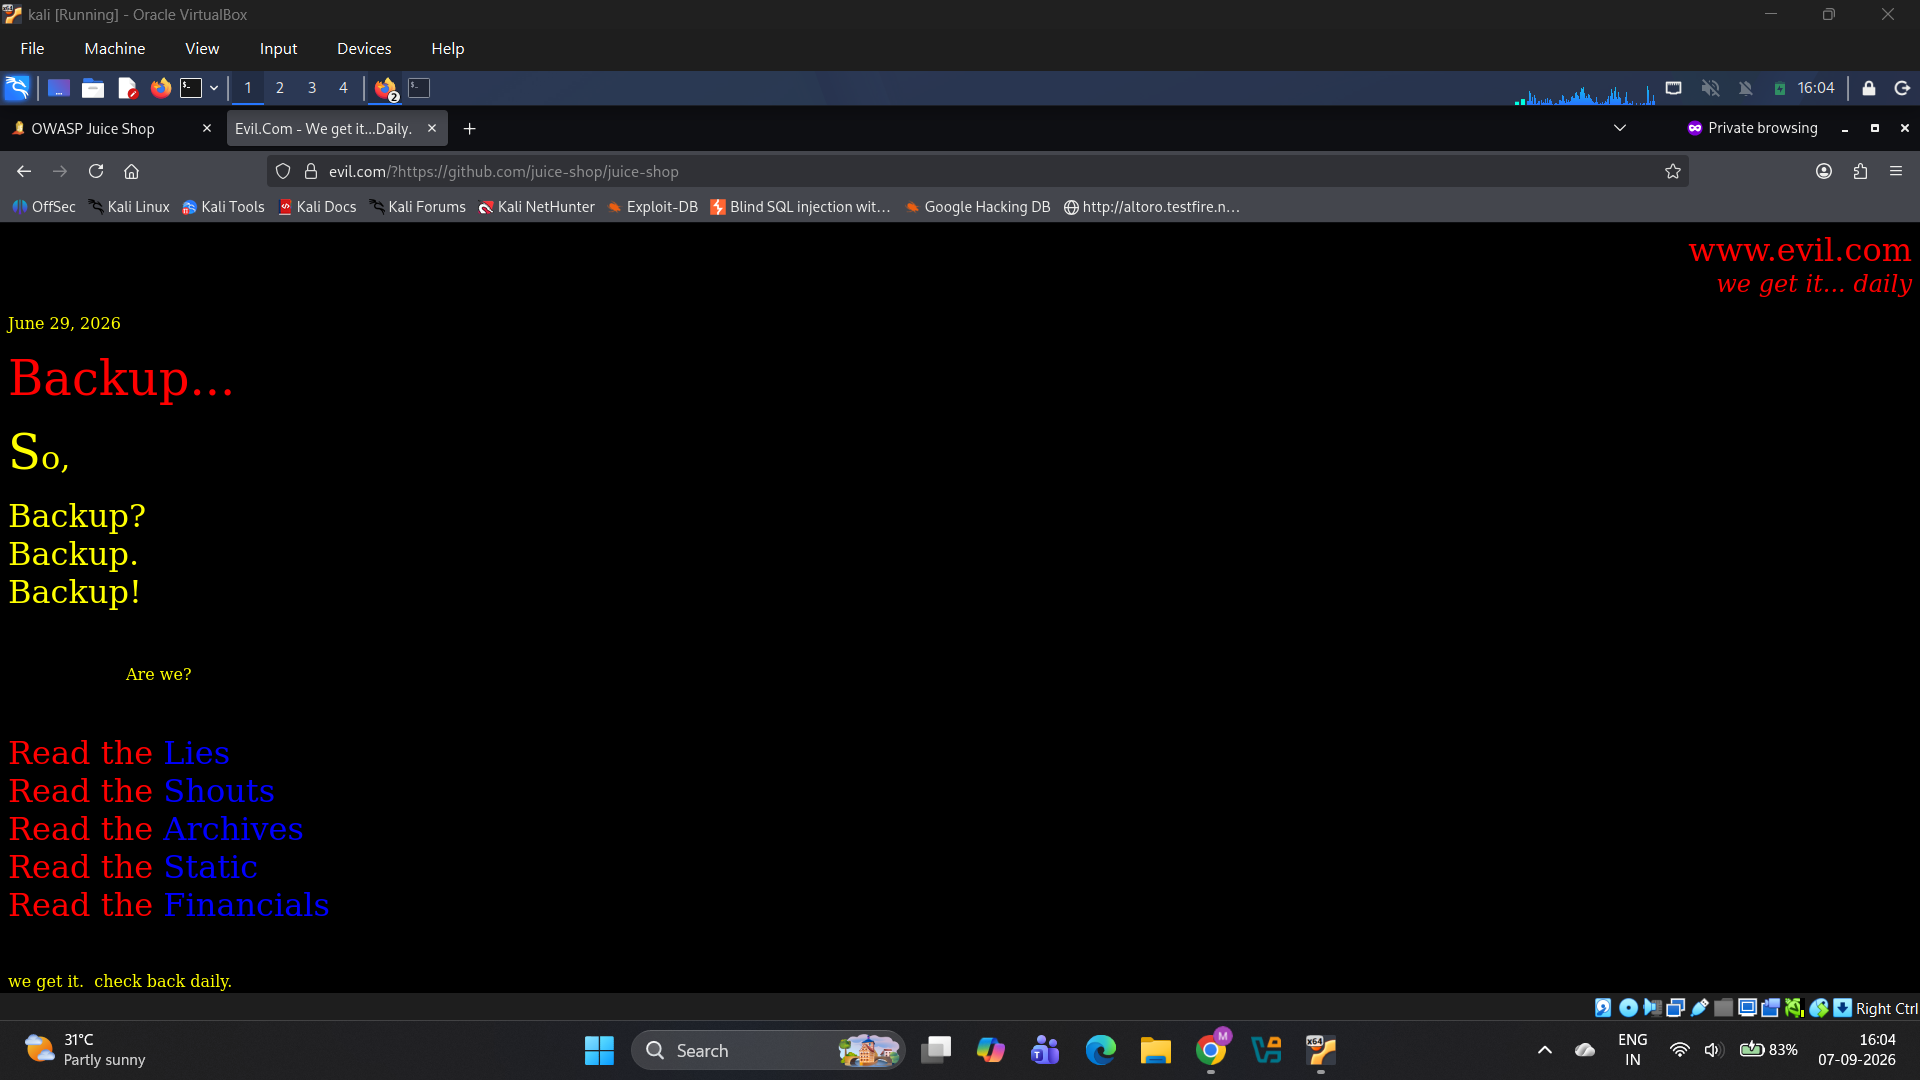
\includegraphics[width=0.8\textwidth]
    {evidence/phase4/openredirect/openredirect-02-manual-bypass-confirmed.png}
    \caption{Manual confirmation of the bypass, redirecting to an untrusted domain}
    \label{fig:openredirect-manual}
\end{figure}

\subsubsection*{Impact}

An attacker can craft a link that begins with the trusted application
domain but ultimately redirects the victim to an attacker-controlled
website.

This can be used in phishing and social engineering attacks, where
the attacker attempts to make the destination appear trustworthy.

Because the initial link uses the trusted application domain, a
victim may be less likely to notice the malicious destination before
following the link.

\subsubsection*{Remediation}

\begin{itemize}

    \item Do not allow the client to control the full redirect
    destination through a URL parameter.

    \item If redirects to external sites are required, validate the
    destination against a strict allowlist of exact, complete domain
    names rather than using substring matching.

    \item Prefer using relative paths for internal redirects instead
    of accepting complete external URLs.

    \item Reject redirect destinations that do not match the
    approved allowlist.

    \item Consider displaying a warning page before redirecting to
    an external domain, allowing the user to confirm the destination.

\end{itemize}

\subsubsection*{Conclusion}

The Open Redirect vulnerability was successfully confirmed through
manual testing. The application allowed an attacker-controlled
destination to bypass the redirect validation and redirect the
browser to an external domain.

The finding is therefore classified as a confirmed Medium-severity
security issue.